%%%%%%%%%%%%%%%%%%%%%%%%%%%%%%%%%%%%%%%%%%%%%%%%%%%%%%%%%%%%%%%%%%%%%%%%%%%%%%%%
%                         FORMATO DE TESIS FI UNAM                             %
%%%%%%%%%%%%%%%%%%%%%%%%%%%%%%%%%%%%%%%%%%%%%%%%%%%%%%%%%%%%%%%%%%%%%%%%%%%%%%%%
% based on Harish Bhanderi's PhD/MPhil template, then Uni Cambridge
% http://www-h.eng.cam.ac.uk/help/tpl/textprocessing/ThesisStyle/
% corrected and extended in 2007 by Jakob Suckale, then MPI-iCBG PhD programme
% and made available through OpenWetWare.org - the free biology wiki

%                     Under GNU License

% ADAPTADO PARA FI-UNAM:  Jesús Velázquez y Marco Ruiz

\documentclass[twoside,11pt]{Latex/Classes/PhDthesisPSnPDF}
%         PUEDEN INCLUIR EN ESTE ESPACIO LOS PAQUETES EXTRA, O BIEN, EN EL ARCHIVO "PhDthesisPSnPDF.cls" EN "./Latex/Classes/"

\usepackage{blindtext}                     % Para insertar texto Lorem ipsum a traves de la etiqueta \blindtext.
\usepackage[]{algorithm2e}                 % Paquete para ulitizar pseudocódigo.
\usepackage{colortbl}
\usepackage{booktabs}
\usepackage{rotating}
\usepackage{multirow}
\usepackage{float}



%%%%%%%%%%%%%%%%%%%%%%%%%%%%%%%%%%%%%%%%%%%%%%
%            Colores de la IPN              %
%%%%%%%%%%%%%%%%%%%%%%%%%%%%%%%%%%%%%%%%%%%%%%
%Azul Pantone 541  -->(0,63,119) RGB
\definecolor{Azul}{RGB}{150,22,2}

%Oro Pantone 460  -->(234,221,150) RGB
\definecolor{Oro}{RGB}{234,221,150}


%%%%%%%%%%%%%%%%%%%%%%%%%%%%%%%%%%%%%%%%%%%%%%
%            Comandos para líneas            %
%%%%%%%%%%%%%%%%%%%%%%%%%%%%%%%%%%%%%%%%%%%%%%
%Se define un comando \colorvrule para hacer líneas verticales de color con 3 argumentos: color, ancho, alto
\newcommand{\colorvrule}[3]{
\begingroup\color{#1}\vrule width#2 height#3
\endgroup}

%Se define un comando \colorhrule para hacer líneas horizontales de color con 2 argumentos: color, ancho
\newcommand{\colorhrule}[2]{
\begingroup\color{#1}\hrule height#2
\endgroup}

%%%%%%%%%%%%%%%%%%%%%%%%%%%%%%%%%%%%%%%%%%%%%%
%          Comando para derivadas            %
%%%%%%%%%%%%%%%%%%%%%%%%%%%%%%%%%%%%%%%%%%%%%%
\newcommand{\derivada}[3][]{\ensuremath{\dfrac{\mbox{d}^{#1}#2}{\mbox{d}#3^{#1}}}} 
%primer argumento(opcional): orden de la derivada
%segundo argumento: función a derivar
%tercer argumento: variable respecto a la que se deriva


%%%%%%%%%%%%%%%%%%%%%%%%%%%%%%%%%%%%%%%%%%%%%%
%       Comando para la exponencial          %
%%%%%%%%%%%%%%%%%%%%%%%%%%%%%%%%%%%%%%%%%%%%%%
\newcommand{\e}[1][]{\ensuremath{\mbox{e}^{#1}}}
%primer argumento(opcional): exponente de la exponencial




% insert a centered figure with caption and description
% parameters 1:filename, 2:title, 3:description and label
\newcommand{\figuremacro}[3]{
	\begin{figure}[htbp]
		\centering
		\includegraphics[width=1\textwidth]{#1}
		\caption[#2]{\textbf{#2} - #3}
		\label{condicion}
	\end{figure}
}

% insert a centered figure with caption and description AND WIDTH
% parameters 1:filename, 2:title, 3:description and label, 4: textwidth
% textwidth 1 means as text, 0.5 means half the width of the text
\newcommand{\figuremacroW}[4]{
	\begin{figure}[htbp]
		\centering
		\includegraphics[width=#4\textwidth]{#1}
		\caption[#2]{\textbf{#2} - #3}
		\label{#1}
	\end{figure}
}

% inserts a figure with wrapped around text; only suitable for NARROW figs
% o is for outside on a double paged document; others: l, r, i(inside)
% text and figure will each be half of the document width
% note: long captions often crash with adjacent content; take care
% in general: above 2 macro produce more reliable layout
\newcommand{\figuremacroN}[3]{
	\begin{wrapfigure}{o}{0.5\textwidth}
		\centering
		\includegraphics[width=0.48\textwidth]{#1}
		\caption[#2]{{\small\textbf{#2} - #3}}
		\label{#1}
	\end{wrapfigure}
}

% predefined commands by Harish
\newcommand{\PdfPsText}[2]{
  \ifpdf
     #1
  \else
     #2
  \fi
}

\newcommand{\IncludeGraphicsH}[3]{
  \PdfPsText{\includegraphics[height=#2]{#1}}{\includegraphics[bb = #3, height=#2]{#1}}
}

\newcommand{\IncludeGraphicsW}[3]{
  \PdfPsText{\includegraphics[width=#2]{#1}}{\includegraphics[bb = #3, width=#2]{#1}}
}

\newcommand{\InsertFig}[3]{
  \begin{figure}[!htbp]
    \begin{center}
      \leavevmode
      #1
      \caption{#2}
      \label{#3}
    \end{center}
  \end{figure}
}







%%% Local Variables:
%%% mode: latex
%%% TeX-master: "~/Documents/LaTeX/CUEDThesisPSnPDF/thesis"
%%% End:
          % Archivo con funciones útiles

%%%%%%%%%%%%%%%%%%%%%%%%%%%%%%%%%%%%%%%%%%%%%%%%%%%%%%%%%%%%%%%%%%%%%%%%%%%%%%%%
%                                   DATOS                                      %
%%%%%%%%%%%%%%%%%%%%%%%%%%%%%%%%%%%%%%%%%%%%%%%%%%%%%%%%%%%%%%%%%%%%%%%%%%%%%%%%
\title{Sistema de plataforma como servicio (PaaS) para la implementación de 
	una mesa de servicio web}
\author{Jose Ricardo Flores Lima}        
\degree{Ingeniero en Telematica}           % Carrera
\director{ \ \ .\ \ \ \ \ \ M.C. y T.E Carlos Hernández Mejía 
	\newline  Dr. Iliac Huerta Trujillo }      % Director de tesiss
\degreedate{2021}                           % Año de la fecha del examen
\lugar{México, CDMX}                        % Lugar
%\portadafalse                              % Portada en NEGRO, descomentar y comentar la línea siguiente si se quiere utilizar
\portadatrue                                % Portada en COLOR

\keywords{tesis,autor,tutor,etc}            % Palablas clave para los metadatos del PDF
\subject{tema_1,tema_2}                     % Tema para metadatos del PDF  

%%%%%%%%%%%%%%%%%%%%%%%%%%%%%%%%%%%%%%%%%%%%%%%%%%%%%
%                   PORTADA                         %
%%%%%%%%%%%%%%%%%%%%%%%%%%%%%%%%%%%%%%%%%%%%%%%%%%%%%
\begin{document}

\begin{titlepage}
\maketitle
\end{titlepage}

%%%%%%%%%%%%%%%%%%%%%%%%%%%%%%%%%%%%%%%%%%%%%%%%%%%%%
%                  PRÓLOGO                          %
%%%%%%%%%%%%%%%%%%%%%%%%%%%%%%%%%%%%%%%%%%%%%%%%%%%%%
%\frontmatter
%\begin{dedication}

\end{dedication}
       % Comentar línea si no se usa
%%\chapter*{}
%\pagenumbering{Roman}

\begin{acknowledgements}



\end{acknowledgements}




   % Comentar línea si no se usa 
%% ******************************* Thesis Declaration ********************************

\begin{declaration}

oihsaiouhiaoushoiuahsiouhasalizado en colaboración, salvo que se indique específicamente en el texto. 
% Author and date will be inserted automatically from thesis.tex
\end{declaration}
           % Comentar línea si no se usa

% Thesis Abstract -----------------------------------------------------


%\begin{abstractslong}    %uncommenting this line, gives a different abstract heading
\begin{abstracts}        %this creates the heading for the abstract page

El continuo crecimiento y desarrollo de las Pequeñas y Medianas Empresas (PyME) dedicadas al soporte técnico e inventarios de infraestructuras de las Tecnologías de la información (TI) de la  Ciudad de México, las ha impulsado a revisar e implementar procesos o métodos de especialización sobre necesidades específicas, que les permitirán marcar una diferencia ante sus competidores.
\newline
El siguiente proyecto presenta como objetivo emplear la guía de las buenas prácticas para la gestión de servicios de tecnologías de la información (ITIL). Esto, a través de la implementación de una mesa de servicio especifica a la necesidad del cliente, la cual sea capaz de gestionar adecuadamente los incidentes y requerimientos que puedan surgir. 
\newline
Para lo anterior, se ha propuesto una aplicación web alojada en la nube mediante la plataforma como servicio (PaaS), complementándose a través de las tecnologías como son el Lenguaje de Consulta Estructurada (SQL), HyperText Markup Language (HTML), Cascading Style Sheets (CSS), JavaScript con su framework Angular.js y Java con su framework Spring Boot. 
\newline
Finalmente, esta tesis pretende ser un aporte para todos aquellos lectores interesados en las vastas herramientas de la informática y quienes además tienen el privilegio de transitar en los pasillos de este honorable Instituto Politécnico Nacional (IPN). 

\begin{center}
	\textbf{Palabras clave: mesa de servicio, PaaS, buenas prácticas ITIL}
\end{center}

\begin{flushright}
	\textbf{\textit{Abstract}}
\end{flushright}

The continuous growth and development of Small and Medium Enterprises (PyME) dedicated to technical support and information technology (IT) infrastructure inventories in Mexico City, has prompted them to review and implement processes or methods of specialization on specific needs, which will allow them to make a difference to their competitors.
\newline
The following project aims to use the best practices guide for information technology service management (ITIL). This, through the implementation of a service desk specific to the client's needs, which is able to adequately manage incidents and requirements that may arise. 
\newline
For the above, it has been proposed a web application hosted in the cloud through the platform as a service (PaaS), complemented through technologies such as Structured Query Language (SQL), HyperText Markup Language (HTML), Cascading Style Sheets (CSS), JavaScript with its framework Angular.js and Java with its Spring Boot framework. 
\newline
Finally, this thesis aims to be a contribution to all those readers interested in the vast tools of computer science and who also have the privilege of walking in the corridors of this honorable Instituto Politécnico Nacional (IPN).

\textbf{\begin{center}
		Keywords: service desk, PaaS, Best Practices ITIL.
\end{center}}

\end{abstracts}
%\end{abstractlongs}


% ----------------------------------------------------------------------                   % Comentar línea si no se usa

%%%%%%%%%%%%%%%%%%%%%%%%%%%%%%%%%%%%%%%%%%%%%%%%%%%%%
%                   ÍNDICES                         %
%%%%%%%%%%%%%%%%%%%%%%%%%%%%%%%%%%%%%%%%%%%%%%%%%%%%%
%Esta sección genera el índice
\setcounter{secnumdepth}{3} % organisational level that receives a numbers
\setcounter{tocdepth}{3}    % print table of contents for level 3
\tableofcontents            % Genera el índice 
%: ----------------------- list of figures/tables ------------------------
\listoffigures              % Genera el ínidce de figuras, comentar línea si no se usa
\listoftables               % Genera índice de tablas, comentar línea si no se usa

%%%%%%%%%%%%%%%%%%%%%%%%%%%%%%%%%%%%%%%%%%%%%%%%%%%%%
%                   CONTENIDO                       %
%%%%%%%%%%%%%%%%%%%%%%%%%%%%%%%%%%%%%%%%%%%%%%%%%%%%%
% the main text starts here with the introduction, 1st chapter,...

\mainmatter
% Thesis Abstract -----------------------------------------------------
%\begin{abstractslong}    %uncommenting this line, gives a different abstract heading
\chapter*{Introducción}
Los sistemas informáticos para la gestión de empresas se han convertido en una herramienta clave en el desarrollo empresarial, necesarias para cumplir los objetivos de los negocios y brindar atención a sus clientes,  Actualmente el mercado ofrece una variedad de herramientas para optimizar los procesos de las PYMES por medio de sistemas de informáticos que capturan, almacenan, procesan y distribuyen la información generada por las distintas unidades administrativas, operativas y productivas de las empresas.\\

Al menos en México existen más de 8 softwares capaces de realizar las actividades previamente mencionadas, pero con un costo elevado [1], Es así como los Sistemas de Planificación de Recursos Empresariales ERP (Enterprise Resource Planning) surgen de la necesidad de integrar todos los datos de una organización, permitiendo obtener información confiable y en tiempo real, desde la fabricación de un producto, pasando por la logística, la distribución, el control de stock, la contabilidad de la organización y demás.\\

En la actualidad la empresa PyME (solicitante del desarrollo de la mesa de servicio) basa su funcionamiento en ERP, sin embargo, requiere una solución que dé respuesta a la gestión, operación y administración de los incidentes que se generan, esta solución deberá adaptarse a la solución ERP con la que cuenta la PyME actualmente.
Nos referiremos a la empresa solicitante de la mesa de servicio como PyME para englobar de manera genérica las características de esta y evitaremos de esta forma utilizar el nombre que por razones de confidencialidad no estamos en posibilidades de mencionarla. Esta empresa tiene más de 8 años dedicada a brindar soluciones integrales de Telecomunicaciones y Administración, hoy cuenta con tres líneas de negocio: en una primera línea se encuentra el proveer capital humano para implementar equipos de cómputo a dependencias Gubernamentales, entenderemos por “implementar equipos de cómputo” como la actividad de cambiar un equipo de cómputo viejo a un nuevo, esta actividad  conlleva la entrega, configuración y documentación pertinente que evalúa el buen funcionamiento del nuevo equipo, en una segunda vertiente se encuentra el soporte técnico a dichos equipos, una vez llevada la fase de implementación se considera un periodo de soporte técnico por un lapso de tiempo el cual esta defino bajo contrato, por lo general estos proyectos constan de 3 años y finalmente una tercera ramificación se encuentra el control de inventarios de equipos de cómputo así como equipos de TI. \\

Por el crecimiento acelerado que ha tenido en los 3 últimos años, el incremento de incidentes ha aumentado de manera acelerada, por lo cual en este momento no cuenta con procesos definidos para la gestión de servicios de incidencias, así mismo carece de un correcto historial de requerimientos, incidentes y cortes de servicio en general. La falta de estos procedimientos repercute en la pérdida de tiempo, recursos e imagen de la PyME.\\

A lo largo de este documento se prende dar una solución integral a la problemática ya expuesta, desarrollando una mesa de servicios bajo las metodologías ITIL, dicha metodología será la base para el desarrollo de una plataforma como servicio (PaaS) que provea una mesa de servicios WEB.
\newpage
 

\def\baselinestretch{1.5}                   % Interlineado de 1.5

% this file is called up by thesis.tex
% content in this file will be fed into the main document
%----------------------- introduction file header -----------------------
%%%%%%%%%%%%%%%%%%%%%%%%%%%%%%%%%%%%%%%%%%%%%%%%%%%%%%%%%%%%%%%%%%%%%%%%%
%  Capítulo 1: Introducción- DEFINIR OBJETIVOS DE LA TESIS              %
%%%%%%%%%%%%%%%%%%%%%%%%%%%%%%%%%%%%%%%%%%%%%%%%%%%%%%%%%%%%%%%%%%%%%%%%%

\chapter{Planteamiento del problema}

%: ----------------------- HELP: latex document organisation
% the commands below help you to subdivide and organise your thesis
%    \chapter{}       = level 1, top level
%    \section{}       = level 2
%    \subsection{}    = level 3
%    \subsubsection{} = level 4
%%%%%%%%%%%%%%%%%%%%%%%%%%%%%%%%%%%%%%%%%%%%%%%%%%%%%%%%%%%%%%%%%%%%%%%%%
%                           Presentación                                %
%%%%%%%%%%%%%%%%%%%%%%%%%%%%%%%%%%%%%%%%%%%%%%%%%%%%%%%%%%%%%%%%%%%%%%%%%

\section{Definición del problema}


%%%%%%%%%%%%%%%%%%%%%%%%%%%%%%%%%%%%%%%%%%%%%%%%%%%%%%%%%%%%%%%%%%%%%%%%%
%                           Def_ Probelma                                    %
%%%%%%%%%%%%%%%%%%%%%%%%%%%%%%%%%%%%%%%%%%%%%%%%%%%%%%%%%%%%%%%%%%%%%%%%%

En la actualidad la empresa realiza funciones de soporte técnico e inventarios  siendo así una de las vertientes del negocio más importantes, por la exposición directa al cliente, la empresa atraviesa  por dificultades con dichos  aspectos debido a la carencia de un software propio que pueda brindar datos en tiempo real de dichos servicios y que a su vez pueda proporcionar un reporteo claro  con datos duros que de pauta a el análisis y a la solución de los incidentes, dado que se cuenta con un impacto directo al SLA (Service Level Agreement) del 21.5\%  de incumplimiento promedio de tiempos de atención asignado, como se muestra en la tabla \ref{tab:PDP1} y la tabla \ref{tab:PDP2} ,  estos incumplimientos provocan penalizaciones, que se estipulan bajo contrato, con la consecuente pérdida de recursos, afectando directamente la imagen de la empresa, con la consecuente pérdida de contratos.

\begin{table}[htbp]
	\centering
	\caption{Representación del SLA de cumplimiento e incumplimiento de tiempos de servicios requeridos estipulados a nivel contrato, zona foránea}
	\scalebox{0.55}{\begin{tabular}{|c|c|c|c|c|c|c|c|}
			\toprule
			\rowcolor[rgb]{ .188,  .329,  .588} \textcolor[rgb]{ 1,  1,  1}{\textbf{Empresa}} & \textcolor[rgb]{ 1,  1,  1}{\textbf{Total dentro del SLA}} & \textcolor[rgb]{ 1,  1,  1}{\textbf{Total fuera del SLA}} & \textcolor[rgb]{ 1,  1,  1}{\textbf{Total de servicios}} & \textcolor[rgb]{ 1,  1,  1}{\textbf{Porcentual }} & \textcolor[rgb]{ 1,  1,  1}{\textbf{Otras areas}} & \textcolor[rgb]{ 1,  1,  1}{\textbf{Total fuera de SLA}} & \textcolor[rgb]{ 1,  1,  1}{\textbf{Total general}} \\
			\midrule
			\multicolumn{1}{|l|}{Diconsa} & 15 & 26 & 41 & \textcolor[rgb]{ 1,  0,  0}{36.5853659} & 87 & 113 & 128 \\
			\midrule
			\multicolumn{1}{|l|}{Fivissste} & 1 & 0 & 1 & \textcolor[rgb]{ 1,  0,  0}{100} & 0 & 0 & 1 \\
			\midrule
			\multicolumn{1}{|l|}{Pemex} & 4 & 0 & 4 & \textcolor[rgb]{ 1,  0,  0}{100} & 0 & 0 & 4 \\
			\midrule
			\multicolumn{1}{|l|}{Pemex PC} & 2 & 0 & 2 & \textcolor[rgb]{ 1,  0,  0}{100} & 3 & 5 & 5 \\
			\midrule
			\multicolumn{1}{|l|}{Prospera} & 43 & 27 & 70 & \textcolor[rgb]{ 1,  0,  0}{61.4285714} & 33 & 60 & 103 \\
			\midrule
			\multicolumn{1}{|l|}{Sedesol } & 31 & 2 & 33 & \textcolor[rgb]{ 1,  0,  0}{93.9393939} & 10 & 12 & 43 \\
			\midrule
			\textcolor[rgb]{ 0,  .69,  .314}{\textbf{Total}} & \textcolor[rgb]{ 0,  .69,  .314}{\textbf{96}} & \textcolor[rgb]{ 0,  .69,  .314}{\textbf{55}} & \textcolor[rgb]{ 0,  .69,  .314}{\textbf{151}} & \textcolor[rgb]{ 0,  .69,  .314}{\textbf{-}} & \textcolor[rgb]{ 0,  .69,  .314}{\textbf{133}} & \textcolor[rgb]{ 0,  .69,  .314}{\textbf{190}} & \textcolor[rgb]{ 0,  .69,  .314}{\textbf{284}} \\
			\bottomrule
		\end{tabular}%
		\label{tab:PDP1}}%
	
\end{table}%

.

  % Table generated by Excel2LaTeX from sheet 'Hoja2'
\begin{table}[htbp]
	\centering
	\caption{Add caption}
\scalebox{0.55}{	\begin{tabular}{|c|c|c|c|c|c|c|c|}
		\toprule
		\rowcolor[rgb]{ .188,  .329,  .588} \textcolor[rgb]{ 1,  1,  1}{\textbf{Empresa}} & \textcolor[rgb]{ 1,  1,  1}{\textbf{Total dentro del SLA}} & \textcolor[rgb]{ 1,  1,  1}{\textbf{Total fuera del SLA}} & \textcolor[rgb]{ 1,  1,  1}{\textbf{Total de servicios}} & \textcolor[rgb]{ 1,  1,  1}{\textbf{Porcentual }} & \textcolor[rgb]{ 1,  1,  1}{\textbf{Otras areas}} & \textcolor[rgb]{ 1,  1,  1}{\textbf{Total fuera de SLA}} & \textcolor[rgb]{ 1,  1,  1}{\textbf{Total general}} \\
		\midrule
		\multicolumn{1}{|l|}{Diconsa} & 15 & 4 & 19 & \textcolor[rgb]{ 1,  0,  0}{78.9473684} & 9 & 13 & 28 \\
		\midrule
		\multicolumn{1}{|l|}{Fivissste} & 13 & 0 & 13 & \textcolor[rgb]{ 1,  0,  0}{100} & 0 & 0 & 13 \\
		\midrule
		\multicolumn{1}{|l|}{Pemex} & 7 & 0 & 7 & \textcolor[rgb]{ 1,  0,  0}{100} & 0 & 0 & 7 \\
		\midrule
		\multicolumn{1}{|l|}{Pemex PC} & 10 & 0 & 10 & \textcolor[rgb]{ 1,  0,  0}{100} & 0 & 0 & 10 \\
		\midrule
		\multicolumn{1}{|l|}{Prospera} & 151 & 31 & 182 & \textcolor[rgb]{ 1,  0,  0}{82.967033} & 31 & 62 & 213 \\
		\midrule
		\multicolumn{1}{|l|}{Sedesol } & 0 & 0 & 0 & \textcolor[rgb]{ 1,  0,  0}{0} & 15 & 15 & 15 \\
		\midrule
		\textcolor[rgb]{ 0,  .69,  .314}{\textbf{Total}} & \textcolor[rgb]{ 0,  .69,  .314}{\textbf{196}} & \textcolor[rgb]{ 0,  .69,  .314}{\textbf{35}} & \textcolor[rgb]{ 0,  .69,  .314}{\textbf{231}} & \textcolor[rgb]{ 0,  .69,  .314}{\textbf{-}} & \textcolor[rgb]{ 0,  .69,  .314}{\textbf{55}} & \textcolor[rgb]{ 0,  .69,  .314}{\textbf{90}} & \textcolor[rgb]{ 0,  .69,  .314}{\textbf{286}} \\
		\bottomrule
	\end{tabular}%
	\label{tab:PDP2}}%
\end{table}%



Derivado de lo antes mencionado, se hace evidente la necesidad de la creación y desarrollo de un software que ayude al aseguramiento, gestión, coordinación y administración de los incidentes.
¿Se puede desarrollar una Mesa de servicio basada en la metodología ITIL, utilizando una plataforma como servicio (PaaS), para dar solución a la gestión, administración y operación de los Incidentes generados en una PyME y que esta se pueda integrar a un ERP?


|	
\section{Justificación}


La PyME solicitante actualmente carece de procesos que integre un software que ayude a ser más eficiente la  gestión de incidentes, ya que las desviaciones que se presentan  al realizarse dichas actividades de forma manual son, la falta de priorización de servicios, carencia de escalación  oportuna, falta de  comunicación, detección de ISSUES (punto de atención) que generen una mejor gestión de los incidentes, así mismo la PyME busca contar con métricas en tiempo real de servicios, ya que al día de hoy  dichas métricas son generadas de forma manual lo cual  cuenta con un margen de error y así mismo se vuelve poco práctico y eficiente, el conjunto de dichas desviaciones antes mencionadas derivan en un incumplimiento de tiempos de servicio requerido o bien en una falta de satisfacción al cliente que a su vez es causante de un impacto económico a nivel proyecto.
La mesa de servicio desarrollada permite gestionar diversos procesos de las incidencias a través de una misma consola y brindar soporte a diferentes tipos de casos como: solicitudes, requerimientos, problemas y cambios, garantizando un manejo eficiente en la gestión del incidente, ofreciendo una respuesta efectiva, lo cual ayudara a mejorar tiempos de operación y de recursos, disminuyendo las perdidas recursos y aumentara la imagen de la Pyme para con sus clientes finales.






\section{Propuesta de solución}

A continuación, se describirá la solución para los diversos problemas que carece la PyME.
\subsection{Mesa de Servicio}
Las principales actividades que desarrollara la Mesa de servicios son: 
•	Optimizar procesos y procedimientos que permitan reducir los tiempos de solución y la correcta escalación de estos.
•	Captación de posibles problemas y solución requerida para los mismos. 
•	Proporcionar a la administración información y recomendaciones para la para la mejora del servicio
•	Generar reportes de los anteriores puntos mencionados.

Considerando las funciones principales de la mesa de servicio se propone como solución la siguiente arquitectura de la figura \ref{fig:DMDS}, donde se atenderán los módulos necesarios para poder satisfacer las necesidades de la PyME.

\begin{figure}[htb]
	\centering
	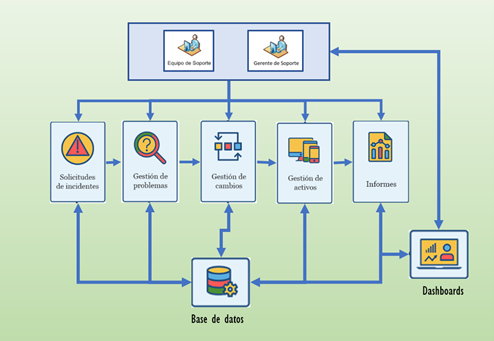
\includegraphics[width=0.9\textwidth]{Capitulo1/Img/MesadeServicioDiagrama}
	\caption{Arquitectura de mesa de servicio, como servicio}
	\label{fig:DMDS}
\end{figure}

\textbf{ Usuarios }

En el siguiente modulo se encuentran el usuario final, referidos como el Equipo de soporte y Gerente de soporte, los cuales tendrán la interacción con la interfaz de sistema con la finalidad de alimentar la base de datos, con los datos necesarios para la gestión correcta de los incidentes.\\

\textbf{Solicitudes de Incidencias }

En este módulo se gestiona y registra la información necesaria para el levantamiento de una solicitud de incidencia el cual dará comienzo al proceso del sistema de mesa de servicio.\\

\textbf{Gestión de problemas }

Durante esta etapa se analizará la información otorgada por el módulo 1.2 para conocer el tipo de incidencias y complejidad de solución y así asignar un nivel de atención.\\

 \textbf{Gestión de cambios.}
 
En este módulo después de un análisis realizado por el personal de soporte en sitio, se evaluará el nivel de atención, de acuerdo con la nueva información recabada y se realizaran los cambios necesarios si así lo amerita.\\

\textbf{Gestión de Activos }

Durante este módulo se realizarán las gestiones de Activos disponibles para poder atender las necesidades de las diversas incidencias.\\

\textbf{ Informes }

En este módulo se genera un medio de consulta diaria, con la finalidad de otorgar visibilidad de las condiciones operativas y administrativas de los incidentes.\\

\textbf{ Base de Datos }

Es el módulo encargado de almacenar, resguardar, organizar y facilitar la información, con el fin de gestionar las incidencias y proporcionar estadistas históricas de estas.

\subsection{Integración de mesa a la plataforma como servicio (PaaS)}


Se propone el desarrollo de un servicio web que integre cada uno de los requerimientos anteriores expuestos en el Figura \ref{fig:DMDS}. En la figura \ref{fig:AMDS} muestra la interacción entre los actores del sistema que, así como la comunicación entre ellos basada en protocolos de comunicación de internet, generando el sistema web de Mesa de Servicio desarrollado con las mejores prácticas.

\begin{figure}[htb]
	\centering
	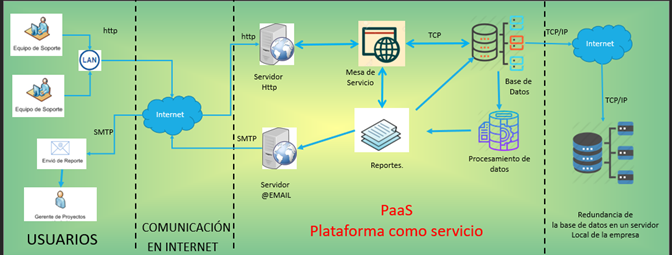
\includegraphics[width=0.9\textwidth]{Capitulo1/Img/AMDS}
	\caption{Intregacion de MS con la arquitectura del sistema como Infraesturura PaaS}
	\label{fig:AMDS}
\end{figure}

 \textbf{Usuarios}
 
Correspondiente al usuarios contendrá a todos los usuarios del sistema, estos realizasen una conexión al servicio web a través de internet con un Localizador Uniforme de Recursos (URL) del hosting que sea asignado al servicio haciendo estas conexiones bajo el protocoló de comunicación HTTP, así mismo tendrán la interacción directa con las interfaces del sistema, que contendrán las herramientas necesarias para la gestión de las atenciones de los servicios de incidencias brindadas por PyME. 
El modulo  usuarios de mesa de servicio se encargará de capturar e ingresar datos al sistema, con esta requisición se enviarán al servicio alojado en la nube.

\textbf{Nube plataforma como servicio (PaaS).}

El módulo  se contendrán al menos 3 subprocesos, alojados en la plataforma como servicio (PaaS) en de algún proveedor de nube ya sea AWS, GOOGLE CLOUD o bien AZURE 
\begin{itemize}

\item \textbf{“Servidor HTTP” }

 será el encargado procesar las solicitudes de conexión a nuestro servicio, así como denegar todas aquellas que no puedan identificarse así mismo todas las solicitudes serán procesadas bajo el protocolo http.
 
\item \textbf{“Mesa de Servicio” }

se encargará de alojar a todo el esquema de codificación del servicio web, estará basado tecnologías web, HTML, JAVA SCRIP Y CSS, este submódulo será el más importante, sus métodos de conexión serán hacia al servidor de Base de datos por el Protocolo TCP.
\item \textbf{“Procesamiento de datos” }
se encargará de llevar a cabo todo el procesamiento de datos contenidos en la base de datos con la finalidad brindar un reporteo de los datos ya mencionados, en este submódulo se implementarán todos los algoritmos de análisis, directamente relacionado con el módulo 1.6.

\item \textbf{“Base de Datos” }
Contendrá la base de Datos con base a un modelo relacional (Base de datos SQL), la interacción entre los módulos de procesamiento de datos y el submódulo de “Mesa de Servicio” se generarán con el protocolo TCP.
\textbf{“Reportes”}
 aunque es una función de los submódulos “procesamiento de información” y “base de datos”, se considera independiente en la arquitectura, por su importancia en el sistema, ya que esta contiene la información ya procesa y con un nivel de utilidad alto para la empresa, así mismo esta   será trasferida a  un submódulo consecuente que a su vez empaquetara y enviara baja el esquema de un correo electrónico, esta función será dirigida por el protocolo SMTP.

\item  \textbf{“Servidor Email”} se encargará de gestionar los correos electrónicos, el lugar donde se almacenan y la forma en la que se envían y reciben mensajes. Su principal función es la de enviar o recibir correos desde un host o servidor hacia distintos destinos a través de internet, la comunicación con internet se hará bajo el proto SMTP.

\end{itemize}


 \textbf{Redundancia de datos en un servidor local} 
 
El ultimo modulo llamado Redundancia de datos en un servidor local, se encargará de generar un respaldo solo de la base de datos del sistema ya que es prioritario tener una copia de seguridad de los datos en un servidor local que no dependa de la infraestructura de la nube, La infraestructura de la nube y en específico el gestor de base de datos harán una conexión con el servidor de la empresa ISAe, bajo los protocolos de comunicación TCP/IP.

\subsection{Integración con ERP}

La empresa PyME solicitante del desarrollo de la mesa de servicio, en la actualidad basa sus actividades en un esquema de ERP, sin embargo, carece de un carece de un servicio que le proporcione la administración, coordinación y gestión de los incidentes, al desarrollar el software como se menciona en los puntos anteriores se da una solución a esta necesidad, sin embargo para lograr tener un optimo desempeño de todo su sistema, la solución de  mesa de servicio será integrado al ERP, como se muestra en la figura \ref{fig:ERP-MDS} .
\begin{figure}[htb]
	\centering
	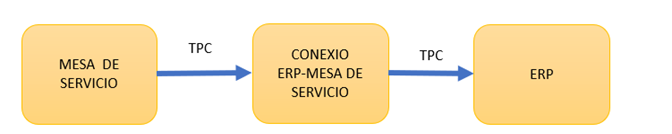
\includegraphics[width=0.9\textwidth]{Capitulo1/Img/ERP-MDS}
	\caption{Implementación de Mesa de Servicio en ERP}
	\label{fig:ERP-MDS}
	
\end{figure}


\textbf{Modulo mesa de servicio.}

El modulo  de  mesa de servicio representa el funcionamiento correcto de forma independiente como servicio y procesos, esta a su vez contara con toda la arquitectura ya antes mencionada en los figura \ref{fig:DMDS} y  la figura \ref{fig:AMDS}.

\textbf{Modulo de conexión }

En este módulo, estará alojada la conexión entre el ERP propiedad de la PyME así como Mesa de servicio desarrollada en esta investigación, esta modulo estará desarrollo con estructura de middleware, esta estará realizada bajo los protocolos de conexión de internet, como lo es TCP.

\textbf{Modulo ERP }

En este módulo se encuentra representada el ERP en el cual basa su funcionamiento la PyME.


\section{Alcances} 
De acuerdo con el desarrollo de solución propuesta se definen los siguientes alcances:
\begin{itemize}
\item Quedan excluidas las siguientes gestiones de la operación de servicio: gestión de acceso y 
gestión de eventos.

\item Quedan excluidas las siguientes disciplinas: estrategia del servicio, diseño del servicio, 
transición del servicio y mejora continua del servicio.

\item La mesa de servicio solo atenderá los  procesos establecidos para la atención, gestión y cierre  de incidencias por la PyME. 

\item Solo se incluirán los roles necesarios para el ciclo de vida de la atención de incidentes.

\item Se incluyen el uso solo de servidores necesarios para el despliegue de la solución propuesta. 

\item El modulo de Redundancia de Datos en un Servidor Local se gestionara solo en las bases de datos.

\item La integración de la mesa al ERP, solo se llevara acabo si el acuerdo de colaboración así lo permite, de no cumplirse, se excluirá de la solución propuesta.
\end{itemize}


\section{Objetivo General} 


Desarrollar una mesa de servicios para una PyME, basada en las mejores prácticas ITIL  e implementada en una plataforma como servicio (PaaS), que permita gestionar, coordinar y administrar incidentes. 


\section{Objetivos específicos} %Escribir al final
\begin{itemize}
	
\item Diseñar la mesa de servicios en base al proceso de desarrollo del catálogo de servicios  aplicando la gestión de niveles de servicio que permita mejorar los procesos de operación para  resolución de peticiones, incidentes y/o problemas.

\item Implementar la función de la mesa de servicios en base al catálogo diseñado, con los acuerdos 
de nivel de servicio y los procesos de operación del servicio establecidos para validar su 
correcto funcionamiento.

\item Desarrollar la mesa de servicio, como servicio web.

\item implementar el desarrollo de mesa de servicio en una plataforma de nube.
\end{itemize}



            % ~10 páginas - Explicar el propósito de la tesis
\include{Capitulo2/Marco_teorico}           % ~20 páginas - Poner un contexto a la tesis, hacer referencia a trabajos actuales en el tema

%%%%%%%%%%%%%%%%%%%%%%%%%%%%%%%%%%%%%%%%%%%%%%%%%%%%%%%%%%%%%%%%%%%%%%%%%
%           Capítulo 3: NOMBRE                   %
%%%%%%%%%%%%%%%%%%%%%%%%%%%%%%%%%%%%%%%%%%%%%%%%%%%%%%%%%%%%%%%%%%%%%%%%%

\chapter{Marco Teórico}
\section{¿Qué es una mesa de Servicio?}
La mesa de Servicio comenzó como un sistema de soporte para solucionar problemas de TI. Fue un trabajo extremadamente técnico centrado en la tecnología en lugar de los usuarios finales. En los primeros días, los servicios de asistencia de TI no tenían que lidiar con ningún tipo de SLA para resolver problemas. No fue hasta ITIL entró en escena que definió y capturó las mejores prácticas de Gestión de Servicios de TI. El modelo de la mesa de servicio de TI centrada en el usuario comenzó a salir a la luz. La mesa de servicio fue vista como un componente necesario del manejo de TI.

Además, los servicios de TI se consideraron un sistema valioso que puede ofrecer respuestas rápidas y reactivas a los problemas del usuario. Y comenzó a ganar una posición única en la industria de TI. Fue utilizado para interactuar y comunicarse diariamente con los consumidores y los empleados. Los datos y las percepciones obtenidas de los problemas técnicos, las elecciones de los usuarios y lo que los usuarios contentos ahora comenzaron a considerarse valiosos para la configuración y el desarrollo de diferentes soluciones de TI. [13]
\subsection{Características de la mesa de servicio}

El principal objetivo de la mesa de servicio es garantizar la satisfacción del cliente. Para ello, se enfoca en evitar fallas, cubrir cuellos de botella y asegurar una prestación de servicios de calidad. Actuando de forma estratégica y preventiva. [14]

Las principales características y funciones de la mesa de servicio son:
\begin{itemize}
	\item 	Actuar como un único punto de contacto para todos los usuarios de los servicios de TI;
\item 	Restablecer el "funcionamiento normal del servicio" lo más rápido posible en caso de una interrupción;
\item 	Rastrear y categorizar preguntas y consultas para ayudar a los gerentes a predecir problemas;
\item 	Apoyar y guiar a la mesa de ayuda desde el principio hasta el final;
\item 	Actuar de forma proactiva para resolver solicitudes complejas de TI;
\item 	Administrar los ciclos de vida del programa, lo que permite un flujo constante de datos;
\item 	Realizar el mantenimiento de todos los sistemas y programas;
\item 	Estudiar e implementar nuevas herramientas tecnológicas que ayuden a asegurar el mejor desempeño de la empresa;
\item 	Administrar los permisos de acceso de los usuarios
\item 	Elaborar informes que muestren y monitoreen el avance del trabajo, verificando que esté alineado con los objetivos predefinidos. 
\end{itemize}

\section{Plataforma como Servicio (PaaS)}
Plataforma como servicio (PaaS) es un entorno de desarrollo e implementación completo en la nube, con recursos que permiten entregar todo, desde aplicaciones sencillas basadas en la nube hasta aplicaciones empresariales sofisticadas habilitadas para la nube. 

El cliente le compra los recursos que necesita a un proveedor de servicios en la nube, a los que accede a través de una conexión segura a Internet, pero solo paga por el uso que hace de ellos.

Al igual que IaaS, PaaS incluye infraestructura (servidores, almacenamiento y redes), pero también incluye middleware, herramientas de desarrollo, servicios de inteligencia empresarial (BI), sistemas de administración de bases de datos, etc. 

PaaS está diseñado para sustentar el ciclo de vida completo de las aplicaciones web: compilación, pruebas, implementación, administración y actualización. 

PaaS permite evitar el gasto y la complejidad que suponen la compra y la administración de licencias de software, la infraestructura de aplicaciones y el middleware subyacentes, los orquestadores de contenedores como Kubernetes, o las herramientas de desarrollo y otros recursos. 
El cliente de nube es el encargado de administrar las aplicaciones y los servicios que desarrolla y, normalmente, el proveedor de servicios en la nube administra todo lo demás. [15]

\subsection{Ventajas de PaaS }

\textbf{Reducir el tiempo de programación}

 Las herramientas de desarrollo de PaaS pueden reducir el tiempo que se tarda en programar aplicaciones nuevas con componentes de aplicación preprogramados que están integrados en la plataforma, como flujos de trabajo, servicios de directorio, características de seguridad, búsqueda, etc. 
 
 \textbf{Agregar más funcionalidad de desarrollo sin incorporar más personal}
  Los componentes de plataforma como servicio pueden aportar a su equipo de desarrollo nuevas características sin necesidad de contratar personal especializado. 
 Desarrollar para varias plataformas (incluidos los dispositivos móviles) con más facilidad. Algunos proveedores de servicios ofrecen opciones de desarrollo para varias plataformas, como PC, dispositivos móviles y exploradores, lo que agiliza y facilita el desarrollo de aplicaciones multiplataforma. 
 
 \textbf{Usar herramientas sofisticadas a un precio asequible}
  Gracias a un modelo de pago por uso, las personas u organizaciones pueden usar software de desarrollo sofisticado y herramientas de inteligencia empresarial y análisis cuya compra no se podrían permitir. 
\textbf{  Colaboración en equipos de desarrollo distribuidos geográficamente}
  Puesto que al entorno de desarrollo se accede a través de Internet, los equipos de desarrollo pueden colaborar en proyectos incluso si los miembros del equipo se encuentran en lugares diferentes. 

 \textbf{Administrar el ciclo de vida de las aplicaciones con eficacia}
  PaaS proporciona todas las características necesarias para sustentar el ciclo de vida completo de las aplicaciones web: compilación, pruebas, implementación, administración y actualización, dentro del mismo entorno integrado. [16]
 
 \section{Servicios Web}
 Los servicios web son aplicaciones autónomas modulares que se pueden describir, publicar, localizar e invocar a través de una red.
 El servidor de aplicaciones da soporte a los servicios web que se desarrollan e implementan de acuerdo con la especificación de servicios web para Java™ EE (Java Platform, Enterprise Edition). El servidor de aplicaciones da soporte a los modelos de programación JAX-WS (Java API for XML Web Services) y JAX-RPC (Java API for XML-based RPC ). JAX-WS es un modelo de programación estratégico que simplifica el desarrollo de aplicaciones mediante el soporte de un modelo estándar basado en anotaciones para desarrollar clientes y aplicaciones de servicios web. [15]
 
 \section{ ITIL }
 
 \subsection{Evolución de ITIL.}
\textbf{Primera versión de ITIL.}

 En su primera versión a finales de la década de 1980, el enfoque inicial de ITIL como marco de trajo fue asegurar que la infraestructura instalada de equipos de cómputo en las organizaciones operara correctamente y con nulo impacto operativo.
 
\textbf{Segunda versión de ITIL V2.}

 Hacia el año 2004 la segunda versión ITIL se centra en promover en las empresas la necesidad de contar con un área de tecnología de información con la asignación de un presupuesto que apoya sus procesos internos con los equipos de cómputo personal y el software para lograr el objetivo de duchas empresas.
 
\textbf{Tercera versión de ITIL V3.}

 La tercera versión de ITIL difundida en 2007 tuvo como enfoque principal mejorar la relación con el cliente y los proveedores del servicio, así como ayudar a las organizaciones en su constante actualización con el apoyo de nuevas tecnologías para obtener mejoras con respecto a ITIL V.2., finalmente se integró la mejora continua como una práctica organizacional, haciendo enfoque a la mejora de procesos, ya establecidos en el marco de trabajo de ITIL y cabe señalar que ITIL V3 tuvo una modificación menor en su proceso en el año 2011.
 
\textbf{Cuarta versión de ITIL V4.}

 Hoy en día y ITIL 4 se enfoca en ofrecer las mejores prácticas en la entrega de servicios considerando las tecnologías y los conceptos de las últimas generaciones en lo que se conoce como transformación digital adaptando nuevas formas de trabajo por ejemplo marcos de trabajo ágiles o de DEVOPS.
 ITIL 4 descansa sobre 2 pilares para por encima de lo que lo que se construyen sus propuestas para una mejor entrega de servicios de tecnologías de la información estas son:
 \begin{itemize}
 	\item El sistema de valor de servicio útil
 	\item	El modelo de cuatro dimensiones de gestión de servicio
 \end{itemize}
 
 A través del sistema de valor de servicios ITIL las organizaciones determinan cómo utilizar los recursos activos y capacidades para que a través del tiempo generen valor a sus clientes en este aspecto es posible decir que el sistema de valor de servicio ITIL cuenta con 5 componentes.
 \begin{enumerate}
 	\item Principio de guía: son recomendaciones que pueden guiar a una organización en cualquier circunstancia independiente de los cambios en su objetivo estrategias tipo de trabajo o estructura de gestión
 	\item	Gobernabilidad:  son los medios por los cual es una organización es dirigida y controlada
 \item Cadena de valor de servicio: es un modelo operativo que describe las actividades clave necesarias para responder a la demanda y facilitar la realización de valor a través de la creación de gestión de productos y servicios.
 	\item	Prácticas: es decir un conjunto de recursos organizacionales diseñados para realizar un trabajo o lograr
 	\item	Mejora continua: es una estrategia organizacional que tiene como objetivo mejorar los productos, servicios, procesos operativos y las relaciones de la organización.
 \end{enumerate}
 
 
 Para conocer mas el marco de trabajo ITIL, se definen lo que para ITIL son conceptos importantes, los  cuales a lo largo del documento se estarán utilizando con la definición propuesta por la misma.
 
 \subsection{¿Qué es un Servicio?}
 Un servicio dentro de la ITIL es el medio que permite la creación conjunta de valor al facilitar los resultados que el cliente desea lograr, sin que éste tenga que administrar costos y riesgos específicos, en otras palabras, a través de los recursos y capacidades se trabaja con los clientes de manera conjunta para determinar la forma en que se resolverán sus problemas y se generará valor en la medida en que se especifica cuál es la utilidad y la garantía de los servicios tienen que cumplir.
 \subsection{¿Qué es la utilidad?}
 La utilidad según ITIL es lo que es un servicio para mejorar el desempeño de un cliente Y/O para eliminar una restricción de un negocio
  \subsection{¿Que son las garantías?}
 Al hablar de garantía se hace referencia a elementos de desempeño tales como.
 \begin{itemize}
 	\item  Capacidad: son las características que tiene un servicio para que un usuario lo pueda utilizar según lo acordado en tiempo y lugar
 	\item Disponibilidad: son las características que tiene un servicio para atender o afrontar adecuadamente la demanda
	\item Seguridad: hace referencia a la protección de los servicios de infraestructura y la información del cliente contra ataques informáticos comprende la integridad la confidencialidad y la durabilidad de la información, así como también integra los procesos de automatización entre dispositivos
	\item continuidad de los servicios: está relacionado con las características que tiene el mismo para que pueda sobrevivir parcial o totalmente encontré un chingo de lana en una pierna
 \end{itemize}


\section{Ciclo de vida del servicio ITIL}
 
 ITIL en su ciclo de vida propone múltiples conceptos, estos a su vez  basándose en el  ciclo de vida del servicio, así mismo incluyendo esencialmente la “Gestión del Servicio” y los conceptos relacionados de “Servicio” y “Valor”. 
 \subsection{Estrategia del Servicio (Service Strategy)}
 las estrategias de servicio proporcionar una guía, tanto a los proveedores de servicios como a sus clientes, con la intención de ayudarles a operar y prosperar, mediante el establecimiento de una estrategia de negocio bien definida.
 Esta fase de estrategia es donde la alta gerencia da luz verde para que inicie un servicio, es decir autorizan si va o no a realizarse un servicio,  por lo cual  en esta fase solo se encuentran a las altas gerencias y mandos medios para la toma de decisiones. 
 

 Esta fase incluye a los procesos siguientes:
 
 \begin{itemize}
 	\item Gestión de Portafolio de Servicios (SPM): En este proceso encontramos a las altas gerencia y mandos medios, esta gestión es netamente administrar los servicios existentes del negocio y tener un histórico de los servicios antiguos. El gerente tiene  visión de sus servicios y conoce la naturaleza de los mismos. 
 	\item 	Gestión Financiera: Agrupa los procesos y actividades asociados con las finanzas de la Gestión del Servicio. Entrega información de gestión indispensable para una operación eficiente y rentable
 \item  Gestión de la Demanda: son los procesos y actividades fundamentales para la gestión del servicio. ya que  permiten determinar la mejor asignación de recursos y  adquisición de artículos.
 	
 \end{itemize}

\subsection{Diseño de Servicio (Service Design, SD)}

 
El diseño de servicios ofrecer pautas para el diseño de servicios apropiados e innovadores, incluyendo su arquitectura, procesos, políticas y documentación, así mismo satisfacer los requisitos de negocio, actuales y futuros, acordados.
 
El objetivo principal es: El diseño de servicios nuevos o modificados, donde se define el alcance para su paso a un entorno de producción.
 
 Los procesos de Diseño del Servicio son: 
 
  
 \begin{itemize}
 	\item \textbf{Gestión del Catálogo de Servicios (SCM)}: El objetivo general es el desarrollo y mantenimiento de un catálogo de servicios que incluya todos los datos precisos y el estado de todos los servicios existentes y de los procesos de negocio a los que apoyan, así como aquellos en desarrollo. 
 	\item  \textbf{Gestión de Niveles de Servicio (SLM):} El objetivo general de este proceso es garantizar que se cumplen los niveles de provisión de los servicios de TI, tanto existentes como futuros, de acuerdo con los objetivos acordados. 
 	\item \textbf{Gestión de la Capacidad}: El objetivo general de este proceso es garantizar que la capacidad se corresponde con las necesidades presentes y futuras del cliente (documentadas en un plan de capacidad).
 	\item  \textbf{	Gestión de la Disponibilidad}: El objetivo general de este proceso es garantizar que los niveles de disponibilidad de los servicios, nuevos o modificados, se corresponden con los niveles acordados con el cliente. Debe mantener el Sistema de Información de gestión de la disponibilidad (AMIS), que es la base del plan de disponibilidad. 
 	 \item\textbf{ Gestión de la Continuidad de los Servicios de TI (ITSCM)}: El objetivo es facilitar la continuidad del negocio (funciones vitales de negocio) garantizando la recuperación de las instalaciones de TI necesarias en el tiempo acordado. 
 	 \item \textbf{Gestión de la Seguridad de la Información}: Garantiza que la política de seguridad de la información satisface los requisitos generales de la organización, así como los que tienen su origen en el gobierno corporativo.
 	\item \textbf{ Gestión de Proveedores}: Este proceso se centra en todos los proveedores y contratos para facilitar la provisión de servicios al cliente.
 	
 \end{itemize}
\subsection{Transición del Servicio (Service Transition, ST)}
En esta fase la operación del servicio cubre la coordinación y ejecución de las actividades y procesos necesarios para entregar y gestionar servicios para usuarios y clientes, con el nivel de servicio acordado. La operación del servicio también tiene la responsabilidad de gestionar la tecnología necesaria para la prestación y el soporte de los servicios.

Los procesos de Transición del Servicio son:
\begin{itemize}
	\item \textbf{Gestión de la Configuración y Activos del Servicio (SACM)}: Gestiona los activos del servicio y elementos de configuración (CIs) para dar soporte a los demás procesos de Gestión del Servicio.
	\item	\textbf{Gestión de Cambios}: Garantiza que los cambios se aplican de una manera controlada,  evaluados, priorizados, planificados, probados, implementados y documentados. 
\item	\textbf{Evaluación del Cambio}: Es un proceso genérico cuyo objetivo consiste en verificar si el rendimiento de algo es aceptable; por ejemplo, si tiene una buena relación calidad/precio, si es continuo, si está en uso, si hay que pagar por ello, etc. 
	\item\textbf{	Gestión de Entregas y Despliegues}: Concentrado en construir, probar y desplegar los servicios especificados en el Diseño del Servicio, y en garantizar que el cliente/usuario puede utilizar el servicio de manera efectiva.
	\item\textbf{	Validación y Pruebas del Servicio}: Las pruebas garantizan que los servicios nuevos o modificados están “ajustados al propósito” y “ajustados al uso”. 
	\item	\textbf{Gestión del Conocimiento}: Mejora la calidad de la toma de decisiones (de la dirección) garantizando la disponibilidad de información segura y fiable durante el Ciclo de Vida del Servicio.
	\item\textbf{ Planificación y Soporte de la Transición}: Garantiza que los recursos se planifican y coordinan adecuadamente para cumplir las especificaciones del Diseño del Servicio.
	
\end{itemize}

\subsection{Operación de Servicio (Service Operation, SO).}

En esta fase la operación del servicio cubre la coordinación y ejecución de las actividades y procesos necesarios para entregar y gestionar los servicios para usuarios y clientes, con el nivel de servicio acordado. La operación del servicio también tiene la responsabilidad de gestionar la tecnología necesaria para la prestación y el soporte de los servicios, esto lo  encontramos en el día a día efectuando la atención a los requerimientos de los clientes y/o usuarios. 

Los procesos de Operación del Servicio son: 

\begin{itemize}
	\item \textbf{Gestión de Peticiones}: Se encarga del tratamiento de peticiones de servicio de los usuarios, proporcionando un canal de solicitud, información y ejecución de la petición. 
\item \textbf{Gestión de Incidencias}: Se concentra en restaurar el fallo del servicio lo antes posible para los usuarios, de manera que su impacto sobre el negocio sea mínimo. 
\item\textbf{ Gestión de Problemas}: Incluye todas las actividades necesarias para diagnosticar las causas subyacentes de las incidencias y para encontrar una solución a esos problemas. 
\item \textbf{Gestión de Eventos}: Supervisa todos los eventos que se producen en la infraestructura de TI con el fin de monitorizar el rendimiento. Este proceso puede estar automatizado para efectuar un seguimiento y escalado ante circunstancias imprevistas.
\item \textbf{Gestión de Accesos}: Permite utilizar el servicio a los usuarios autorizados y limita el acceso a los usuarios sin autorización.
	
\end{itemize}


\subsection{Mejora Continua del Servicio (Continuous Service Improvement, CSI).}

Los departamentos de TI tienen que mejorar continuamente sus servicios para seguir atendiendo al llamamiento del negocio. De esto se ocupa la fase de Mejora Continua del Servicio (CSI) del ciclo de vida.
Se debería aplicar CSI a lo largo de todo el ciclo de vida, en todas sus fases, desde la Estrategia a la Operación. En este sentido, se convierte en algo inherente tanto al desarrollo como a la provisión de servicios de TI.
  % ~20 páginas - Explicar el problema en específico que se va a resolver, la metodología y experimentos métodos utilizados
\chapter{Análisis y Diseño}
Para desarrollar un sistema de calidad se necesita requerimientos hechos por el cliente, los cuales están proporcionados, por la PyME solicitante del sistema, la etapa de análisis y diseño estarán desarrolladas por módulos. 

El siguiente análisis estará compuesto por:

\begin{itemize}
	\item Especificación de requerimientos 
	\item 	Modelo de comportamiento
	\begin{itemize}
		\item Modelo de procesos 
		\begin{itemize}
			\item	Diagrama de frujo 
			\item 	Diccionario de datos 
		\end{itemize}
	\item Modelo de datos
	\begin{itemize}
		\item Diagrama de entidad Relación
	\end{itemize}
	
	\end{itemize}
	
		\item Interfaz gráfica de usuario.
\end{itemize}





    \section{Requerimientos  del sistema}
    
   En este sección  contiene los requerimientos que serán necesarios para el correcto funcionamiento del software de mesa de servicio. 
   Los requerimientos solo serán mencionados el secciones posteriores se describirán puntualmente cada uno de ellos.

\subsection{Requerimientos no funcionales }


\begin{itemize}
	\item Portafolio de servicio
	\item Categorización de servicio 
	\item Matriz de urgencia e impacto 
	\item Acuerdos de nivel de servicio (SLA).
	\item Roles y puestos de mesa de servicio.
	\item Seguridad
	\item Disponibilidad
	
\end{itemize}

\subsubsection{Portafolio de servicio}
Actualmente la PyME se encuentra en un planteamiento de apertura de nuevo portafolio de servicios, sin embrago en la actualidad cuenta con las siguientes descripciones de servicios como se puede ver en la tabla \ref{tab:CatSer}.

  % Table generated by Excel2LaTeX from sheet 'Portafolio de servicos '
\begin{table}[H]
	\centering
	\caption{Descripción de portafolio de servicio}
	\scalebox{0.55}{	\begin{tabular}{|p{17.57em}|p{64.715em}|}
		\toprule
		\rowcolor[rgb]{ .122,  .22,  .392} \textcolor[rgb]{ 1,  1,  1}{SERVICIO} & \textcolor[rgb]{ 1,  1,  1}{DESCRIPCIÓN DE SERVICIO} \\
		\midrule
		Administración de servidores & Administración de Centros de Computo e infraestructura tecnológica.\newline{}Instalación, configuración, mantenimiento. correctivo y preventivo.\newline{}Administración de servidores Linux,. Windows Server, Asterisk, directorio activo, correo electrónico.\newline{}Realizamos migraciones de Sistemas. Operativos.\newline{} \\
		\midrule
		Venta y renta de equipo de cómputo. & Venta y renta de equipo de computo laptop, CPU \newline{}Venta y renta de perifericos de equipos de laptop y CPU \newline{}Parner de HP, DELL, LENOVO, APPLE,  \\
		\midrule
		Mesa de servicio  & Al llamar a la mesa de ayuda, el usuario indica su problema y el agente receptará su petición y generará el ticket correspondiente, si se necesita la presencia física del técnico se escalará al siguiente nivel para que el soporte 2 realice la visita técnica reasignando así el ticket de atención. \\
		\bottomrule
	\end{tabular}%
	\label{tab:CatSer}}%
\end{table}%
\subsubsection{Categorización de servicios}
En la siguiente sección se define el  conjunto completo de servicios, los cuales forman parte el portafolio de servicios de la PyME, sin embargo el análisis de la categorización de servicios solo implicara el servicio de “mesa de servicio”. 
La categorización de servicios se realiza en dos segmentos los cuales son:
\begin{itemize}
	\item Incidente
	\item Requerimientos. 
\end{itemize}


En la tabla \ref{tab:INCSOF} podemos observar los incidentes correspondientes a software así como el servicio que proporciona TI a dichos incidentes.




   % Table generated by Excel2LaTeX from sheet 'programas '
 \begin{table}[H]
 	\centering
 	\caption{Incidentes de tipo Software}
 	\scalebox{0.55}{\begin{tabular}{|c|c|l|c|}
 		\toprule
 		\rowcolor[rgb]{ .267,  .447,  .769} \textcolor[rgb]{ 1,  1,  1}{Tipo de servicio} & \textcolor[rgb]{ 1,  1,  1}{Categoria} & \multicolumn{1}{c|}{\textcolor[rgb]{ 1,  1,  1}{Subcategoria}} & \textcolor[rgb]{ 1,  1,  1}{Servicios de IT} \\
 		\midrule
 		\multirow{15}[29]{*}{\begin{turn}{-90}INCIDENTE  \end{turn}} & \multirow{15}[29]{*}{\begin{turn}{-90}PROGRAMAS \end{turn}} & Outlook & \multicolumn{1}{c|}{\multirow{15}[29]{*}{* Instalación\newline{}\newline{}* Activación licencia\newline{}\newline{}* Actualización}} \\
 		\cmidrule{3-3}        &   & Word  &  \\
 		\cmidrule{3-3}        &   & Excel &  \\
 		\cmidrule{3-3}        &   & PowerPoint &  \\
 		\cmidrule{3-3}        &   & Visio &  \\
 		\cmidrule{3-3}        &   & AutoCAD &  \\
 		\cmidrule{3-3}        &   & SAP &  \\
 		\cmidrule{3-3}        &   & Antivirus &  \\
 		\cmidrule{3-3}        &   & SQL server &  \\
 		\cmidrule{3-3}        &   & Acrobat &  \\
 		\cmidrule{3-3}        &   & Java &  \\
 		\cmidrule{3-3}        &   & Visual studio &  \\
 		\cmidrule{3-3}        &   & Office 365 &  \\
 		\cmidrule{3-3}        &   & Google crome  &  \\
 		\cmidrule{3-3}        &   & Internet explore   &  \\
 	\end{tabular}%
 	\label{tab:INCSOF}}%
 \end{table}%

.
En la  tabla \ref{tab:INCHAR}, se describen los incidentes, con una subcategorización de hardware,  donde se describen los servicios proporcionados por el departamento de IT. 

  % Table generated by Excel2LaTeX from sheet 'Harware '
\begin{table}[H]
	\centering
	\caption{Incidentes de tipo hardware}
	\scalebox{0.55}{\begin{tabular}{|c|c|l|c|}
		\toprule
		\rowcolor[rgb]{ .267,  .447,  .769} \textcolor[rgb]{ 1,  1,  1}{Tipo de servicio} & \textcolor[rgb]{ 1,  1,  1}{Categoria} & \multicolumn{1}{c|}{\textcolor[rgb]{ 1,  1,  1}{Subcategoria}} & \textcolor[rgb]{ 1,  1,  1}{Servicios de IT} \\
		\midrule
		\multirow{13}[26]{*}{\begin{turn}{-90}I N C I D E N T E  \end{turn}} & \multirow{13}[26]{*}{\begin{turn}{-90}H A R W A R E \end{turn}} & Laptop / portatil  & \multicolumn{1}{c|}{\multirow{13}[26]{*}{Instalación\newline{}Falla\newline{}Cambio de sitio\newline{}Configuración \newline{}Reposición \newline{}Mantenimiento}} \\
		\cmidrule{3-3}        &   & Pc &  \\
		\cmidrule{3-3}        &   & Monitor &  \\
		\cmidrule{3-3}        &   & Teclado &  \\
		\cmidrule{3-3}        &   & Mouse  &  \\
		\cmidrule{3-3}        &   & Lector de DVD  &  \\
		\cmidrule{3-3}        &   & Impresora &  \\
		\cmidrule{3-3}        &   & Escáner  &  \\
		\cmidrule{3-3}        &   & Disco duro interno /externo   &  \\
		\cmidrule{3-3}        &   & Proyector  &  \\
		\cmidrule{3-3}        &   & Proyector  &  \\
		\cmidrule{3-3}        &   & Pantallas /tv &  \\
		\cmidrule{3-3}        &   & UPS &  \\
		\bottomrule
	\end{tabular}%
	\label{tab:INCHAR}}%
\end{table}%




Dentro del servicio a proporcionar se consideran dos tipos de servicios, soporte técnico y administrativos de control, donde se incluirá dentro de administrativos de control la sub categoría requerimiento la cual se define como todo aquel servicio que no represente una falla.

A continuación en la siguiente tabla \ref{tab:REAADM} se presenta la descripción de los requerimientos, que se estarán proporcionando como servicio de atención. 


  % Table generated by Excel2LaTeX from sheet 'REQUERIMIENTO'
\begin{table}[h!]
	\centering
	\caption{Categorización de requerimientos de procesos administrativos }
\scalebox{0.55}{	\begin{tabular}{|c|c|r|r|}
		\toprule
		\rowcolor[rgb]{ .267,  .447,  .769} \textcolor[rgb]{ 1,  1,  1}{Tipo de servicio} & \textcolor[rgb]{ 1,  1,  1}{Categoria} & \multicolumn{1}{c|}{\textcolor[rgb]{ 1,  1,  1}{Subcategoria}} & \multicolumn{1}{c|}{\textcolor[rgb]{ 1,  1,  1}{Servicios de IT}} \\
		\midrule
		\multirow{18}[36]{*}{\begin{turn}{-90}Requerimiento \end{turn}} & \multirow{18}[36]{*}{\begin{turn}{-90}Procesos Administrativo.\end{turn}} & \multicolumn{1}{r|}{\multirow{10}[20]{*}{Implementación de equipo de cómputo/ alta de equipo    }} & Configuración de dominio  \\
		\cmidrule{4-4}        &   &   & Configuración de red  \\
		\cmidrule{4-4}        &   &   & Configuración de perfil del usuario  \\
		\cmidrule{4-4}        &   &   & Configuración de Impresoras \\
		\cmidrule{4-4}        &   &   & Migración de información  \\
		\cmidrule{4-4}        &   &   & Configuración de carpetas compartidas \\
		\cmidrule{4-4}        &   &   & Configuración de PST  \\
		\cmidrule{4-4}        &   &   & Configuración de aplicativos  \\
		\cmidrule{4-4}        &   &   & Configuración de correo electrónico  \\
		\cmidrule{4-4}        &   &   & Creación de resguardo  \\
		\cmidrule{3-4}        &   & \multicolumn{1}{r|}{\multirow{3}[6]{*}{Borrado y retiro de equipo de cómputo / baja de equipo  }} & Borrado seguro  \\
		\cmidrule{4-4}        &   &   & Validación de certificado de borrado  \\
		\cmidrule{4-4}        &   &   & Baja de resguardo de equipo de computo  \\
		\cmidrule{3-4}        &   & \multicolumn{1}{r|}{\multirow{3}[6]{*}{Actualización de resguardo }} & Validación de componentes del equipo   \\
		\cmidrule{4-4}        &   &   & Actualización de datos del equipo  \\
		\cmidrule{4-4}        &   &   & Actualización de datos de usuario  \\
		\cmidrule{3-4}        &   & \multicolumn{1}{r|}{\multirow{2}[4]{*}{Reubicacion }} & Actulizacion de datos del usuario  \\
		\cmidrule{4-4}        &   &   & Actulizacion de Informacion de ubicación  \\
		\bottomrule
	\end{tabular}%
	\label{tab:REAADM}}%
\end{table}%



\subsubsection{Matriz de urgencia e impacto}

Dentro de las buenas prácticas de ITIL para la gestión de incidentes es necesario establecer una matriz de prioridad en función a la urgencia e impacto, cual  permita establecer tiempos de atención en los incidentes como se muestra en la tabla \ref{tab:MATURG}.
  % Table generated by Excel2LaTeX from sheet 'Hoja6'
\begin{table}[H]
	\centering
	\caption{Matriz de urgencia e impacto}
	\begin{tabular}{|c|c|p{31.145em}|}
		\toprule
		\rowcolor[rgb]{ .267,  .447,  .769} \multicolumn{3}{|c|}{\textcolor[rgb]{ 1,  1,  1}{Definición de impacto}} \\
		\midrule
		\rowcolor[rgb]{ .267,  .447,  .769} \textcolor[rgb]{ 1,  1,  1}{Nivel} & \textcolor[rgb]{ 1,  1,  1}{Valor} & \multicolumn{1}{c|}{\textcolor[rgb]{ 1,  1,  1}{Descripción}} \\
		\midrule
		Alto & Impacto 3 & El equipo o servicio no se encuentra disponible u trabaja con algunas restricciones perjudicando de manera masiva o colando en riesgo el servicio. Se atiende de forma prioritaria de acuerdo a los SLA pactados. \\
		\midrule
		mediano & Impacto 2 & El usuario no puede trabajar derivado del fallo de el equipo, sistema o aplicativo importante para la operación y finalización de un trabajo \\
		\midrule
		Bajo & Impacto 1 & El equipo, sistema o aplicativo trabaja con algunas restricciones. El Impacto es mínimo el usuario. El problema no manifiesta riesgo o impacto en la finalización de un trabajo. \\
		\bottomrule
	\end{tabular}%
	\label{tab:MATURG}%
\end{table}%



\subsubsection{Nivel de servicio}
El acuerdo de nivel de servicio (Service Level Agreement, SLA), es un documento resultante de la Gestión del Nivel de Servicio (de la Disciplina Diseño del Servicio), y representa el acuerdo entre un cliente y un proveedor de servicios de TI. Este SLA, especifica un servicio de TI, con sus objetivos de nivel de servicio y las responsabilidades del proveedor de servicios de TI y del cliente. Se debe comprender que el SLA es una extensión de los servicios del Catálogo de Servicios, ya que define principalmente las metas de atención de estos en base a una prioridad, grupo de cliente(s) a quien se ofrece el servicio y responsabilidades mutuas. En definitiva, el SLA se define desde el punto de vista del cliente que tenga que ser atendido.

Actualmente la empresa cuenta con dos tipos de SLA’s, el primer SLA referirá al primer contacto con el usuario, dando por consecuencia el segundo SLA, si es dado caso que no se pudiera atender el requerimiento o incidente según sea el caso, dentro del primero SLA, los SLA’s se estarán dado en horas como se muestra en la tabla \ref{tab:SLA1}.


  % Table generated by Excel2LaTeX from sheet 'Hoja7'
\begin{table}[H]
	\centering
	\caption{Niveles de SLA}

\scalebox{0.60}{	 \begin{tabular}{|r|r|r|r|r|}
	\toprule
	\rowcolor[rgb]{ .184,  .329,  .588} \textcolor[rgb]{ 1,  1,  1}{\textbf{Prioridad}} & \textcolor[rgb]{ 1,  1,  1}{\textbf{Tiempo de Respuesta}} & \textcolor[rgb]{ 1,  1,  1}{\textbf{Tiempo en solución (hrs)}} & \textcolor[rgb]{ 1,  1,  1}{\textbf{Tiempo Total (hrs)}} & \textcolor[rgb]{ 1,  1,  1}{\textbf{Servicio}} \\
	\midrule
	\multicolumn{1}{|c|}{\multirow{2}[4]{*}{Critico}} & \multicolumn{1}{c|}{\multirow{2}[4]{*}{2}} & \multicolumn{1}{c|}{\multirow{2}[4]{*}{16}} & \multicolumn{1}{c|}{\multirow{2}[4]{*}{18}} & \multicolumn{1}{p{19.855em}|}{Incidencia} \\
	\cmidrule{5-5}        &   &   &   & \multicolumn{1}{p{19.855em}|}{Requerimiento } \\
	\midrule
	\multicolumn{1}{|c|}{\multirow{2}[4]{*}{Alto}} & \multicolumn{1}{c|}{\multirow{2}[4]{*}{18}} & \multicolumn{1}{c|}{\multirow{2}[4]{*}{24}} & \multicolumn{1}{c|}{\multirow{2}[4]{*}{52}} & \multicolumn{1}{p{19.855em}|}{Incidencia} \\
	\cmidrule{5-5}        &   &   &   & \multicolumn{1}{p{19.855em}|}{Requerimiento } \\
	\midrule
	\multicolumn{1}{|c|}{\multirow{2}[4]{*}{Bajo}} & \multicolumn{1}{c|}{\multirow{2}[4]{*}{48}} & \multicolumn{1}{c|}{\multirow{2}[4]{*}{120}} & \multicolumn{1}{c|}{\multirow{2}[4]{*}{168}} & \multicolumn{1}{p{19.855em}|}{Incidencia} \\
	\cmidrule{5-5}        &   &   &   & \multicolumn{1}{p{19.855em}|}{Requerimiento } \\

	\bottomrule
\end{tabular}%

	\label{tab:SLA1}}%
\end{table}%


\subsubsection{Roles y puesto de mesa de servicio}

La organización en una empresa es necesaria e indispensable ya deben aportar a las personas y trabajadores la cultura de la empresa, detallando y clarificando las estrategias y los objetivos del negocio, para lo cual el personal debe tener una visión clara sobre su misión, rol, implicación y contribución dentro del proceso del servicio.

Para ITIL las personas son los elementos clave de una de sus dimensiones, donde  agrupa a todo el personal implicado en la entrega del servico y no únicamente la entidad de informática, por lo cual ITIL como marco de referencia sugiere para el desarrollo de una mesa de servicio pensando el personal que al momento de diseñar un servicio, se definan que responsabilidades tendrá dicho rol para determinar la autoridad adecuada, así mismo asignar identificar si el rol será asignado a uno o más personas. 

A continuación, una breve descripción del personal que forma parte en la atención y gestión de una Mesa de servicios.

\textbf{Service desk manager (gerente de mesa de servicio)}



El service desk manager se encarga de coordinar el equipo de la mesa de servicios, mantener la coordinación entre las partes involucradas. 

Un service desk manager es el responsable de que los servicios se entreguen de manera oportuna y también sirve como enlace de la mesa de servicio para la ejecución de las principales iniciativas que impactan el negocio.

Es el encargado de Supervisar el personal a su cargo y evaluará algunos aspectos como:

\begin{itemize}
	\item 	Evaluación de desempeño del personal.
\item 		Organizar y planificar las actividades con los agentes de cuentas.
	\item 	Cumplir los procedimientos de la Mesa de Servicios y asegurarse que su personal a cargo lo realice.
\item 		Realizar estadísticas de incidentes.
\item 		Dar seguimiento de las tareas asignadas a cada agente.
\item 		Administrar los incidentes, pedidos o reclamos recibidos sobre los servicios atendidos.
\item 		Emitir informe de servicios semanal y mensual.
\item 		Contribuir al desarrollo de los manuales de normas y procedimientos, detectar necesidades de capacitación de los miembros de su equipo.
	
\end{itemize}

\textbf{Coordinador de la mesa de servicio}

Es el encargado de:
\begin{itemize}
\item Supervisar las actividades incluidas en los servicios.
\item Asegurar el nivel de servicio, gestión y organización del equipo de trabajo.
\item Aplicar las mejores prácticas definidas por ITIL. 
\item Mantener una actitud proactiva frente a las oportunidades de mejora de los servicios.
\item Coordinar la realización de la encuesta de satisfacción del servicio.
\item Detectar necesidades de capacitación del personal.

\end{itemize}
\textbf{Agentes de la mesa de servicio}

Es el encargado de recibir llamadas o correos por los usuarios de los clientes de la empresa donde:


\begin{itemize}
\item Exista interrupción no planificada o reducción de la calidad del servicio
\item Interrumpa la operación normal de trabajo.
\item Requerimiento de soporte sobre el software y hardware a primer nivel.
\item Efectúen consultas planteadas por usuarios, distintos tipos de asesoramientos en el funcionamiento y utilización de los recursos informáticos.
\item Identificar los problemas, primera instancia de llamada 
\item Confirmar la satisfacción del usuario con respecto a la solución brindada.
\item Levantamiento de Incidencias.

\end{itemize}
\textbf{Técnicos de la mesa de servicio}

Es el encargado de:
\begin{itemize}
	\item Ejecutar trabajos de mantenimiento preventivo y correctivo de los equipos de computación.
	\item Brindar el soporte oportuno en los sistemas informáticos, que comprende lo siguiente
	\begin{itemize}
			\item Mantenimiento e implantación de software.
		\item Mantenimiento de base de datos de usuarios y correos.
		
	\end{itemize}

	\item Capacitar en el uso de herramientas.
	\item Documentar las soluciones dadas para mantener actualizado el Catálogo de Servicio.
	
\end{itemize}


Para realizar una mejor interpretación de los roles de trabajo,  se presenta un modelo RACI  donde se especifica la interacción que tiene cada uno de los roles a participar en el servicio, como se muestra en la tabla \ref{tab:RACI}.

  % Table generated by Excel2LaTeX from sheet 'Hoja8'
\begin{table}[htbp]
	\centering
	\caption{Modelo RACI de roles}
\scalebox{0.55}{	     
	\begin{tabular}{|p{15.355em}|p{11.215em}|p{13.645em}|p{17.285em}|p{14.355em}|}
		\toprule
		\rowcolor[rgb]{ .184,  .329,  .588} \multicolumn{1}{|r|}{\textcolor[rgb]{ 1,  1,  1}{}} & \multicolumn{1}{r|}{\textcolor[rgb]{ 1,  1,  1}{\textbf{Agentes de la mesa}}} & \multicolumn{1}{r|}{\textcolor[rgb]{ 1,  1,  1}{\textbf{Gerente de mesa}}} & \multicolumn{1}{r|}{\textcolor[rgb]{ 1,  1,  1}{\textbf{Coordinador de la mesa}}} & \multicolumn{1}{r|}{\textcolor[rgb]{ 1,  1,  1}{\textbf{Técnicos de la mesa }}} \\
		\midrule
		Apertura de Ticket & \textbf{C} & \multicolumn{1}{c|}{} & \textbf{I} & \multicolumn{1}{c|}{} \\
		\midrule
		Documentación de Incidente & \textbf{R} & \multicolumn{1}{c|}{} & \textbf{A} & \multicolumn{1}{c|}{} \\
		\midrule
		Asignación de Incidente & \textbf{R} & \textbf{A} & \textbf{R} & \textbf{C} \\
		\midrule
		Análisis de incidentes & \textbf{C} & \textbf{I} & \textbf{I} & \textbf{R/A} \\
		\midrule
		Escalamiento de incidente & \textbf{I} & \textbf{I} & \textbf{I} & \textbf{R/A} \\
		\midrule
		Cierre de ticket & \textbf{C} & \textbf{I} & \textbf{I} & \textbf{R/A} \\
		\bottomrule
	\end{tabular}%
	\label{tab:RACI}}%
\end{table}%

\section{Requerimientos funcionales}




\begin{itemize}
	\item Módulo de Registro y levantamiento de incidentes.
\end{itemize}   % ~20 páginas - Presentar los resultados tal cual son, y analizarlos.
\include{Capitulo5/Conclusiones}            % ~5 páginas - Resumir lo que se hizo y lo que no y comentar trabajos futuros sobre el tema

%%%%%%%%%%%%%%%%%%%%%%%%%%%%%%%%%%%%%%%%%%%%%%%%%%%%%
%                   APÉNDICES                       %
%%%%%%%%%%%%%%%%%%%%%%%%%%%%%%%%%%%%%%%%%%%%%%%%%%%%%
\appendix
\include{Apendice1/Apendice1}               % Colocar los circuitos, manuales, código fuente, pruebas de teoremas, etc.

%%%%%%%%%%%%%%%%%%%%%%%%%%%%%%%%%%%%%%%%%%%%%%%%%%%%%
%                                     %
%%%%%%%%%%%%%%%%%%%%%%%%%%%%%%%%%%%%%%%%%%%%%%%%%%%%%
\begin{small} % tiny(5) < scriptsize(7) < footnotesize(8) < small (9)
\bibliographystyle{Latex/Classes/PhDbiblio-url2}    % Title is link if provided
\bibliography{Bibliografia/Referencias}             % Archivo .bib
\end{small}
% --------------------------------------------------------------
% existen varios estilos de bilbiografía, pueden cambiarlos a placer

% in-text refs: (1) (1; 2)
% ref list: alphabetical; author(s) in small caps; initials last name; page(s)
%\bibliographystyle{Latex/Classes/PhDbiblio-case} % title forced lower case
%\bibliographystyle{Latex/Classes/PhDbiblio-bold} % title as in bibtex but bold
%\bibliographystyle{Latex/Classes/PhDbiblio-url} % bold + www link if provided

%\bibliographystyle{Latex/Classes/jmb} % calls style file jmb.bst
% in-text refs: author (year) without brackets
% ref list: alphabetical; author(s) in normal font; last name, initials; page(s)

%\bibliographystyle{plainnat} % calls style file plainnat.bst
% in-text refs: author (year) without brackets
% (this works with package natbib)
% --------------------------------------------------------------
% according to Dresden med fac summary has to be at the end
%\include{0_frontmatter/abstract}
%: Declaration of originality
%\include{9_backmatter/declaration}

\end{document}